\documentclass[a4paper]{report}
\usepackage[T1]{fontenc}
\usepackage[utf8]{inputenc}
\usepackage{lmodern}
\usepackage{graphicx}
\usepackage[left=3cm,right=3cm,top=3cm,bottom=3cm]{geometry}
\usepackage{eurosym}
\usepackage{fancyhdr}%encabezado y pie de página
\usepackage[colorlinks=true, linkcolor=black, urlcolor=blue]{hyperref}
\setcounter{secnumdepth}{5}
\usepackage[spanish]{babel}
\setcounter{tocdepth}{5}
\usepackage{colortbl}%para colorear tablas
\usepackage{tabularx}
\usepackage{pdfpages}%para incluir documentos pdf
\usepackage{placeins}%para poner barrera y no pasen de secciones los elemntos flotantes
\usepackage{longtable}
\usepackage{multirow} %para juntar varias filas en una tabla
\usepackage{rotating}

\author{Andoni Martín Reboredo \\ David Ramirez Ambrosi}
\title{\begin{center}
\textbf{\Huge{Práctica 6, Clustering}} \\ 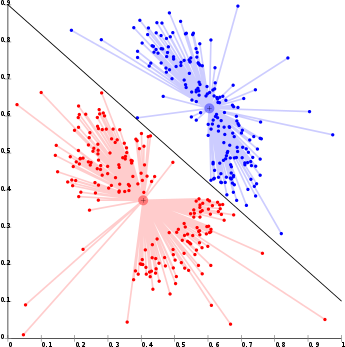
\includegraphics{./Figuras/KMeans-density-data.png}\\  \textbf{Minería de datos}
\end{center}}
\date{\today}



\pagestyle{fancy}
\rhead{
\textbf{Minería de datos} \hfill Práctica 6: Clustering
}

\lhead{}

%colores
\definecolor{azul}{RGB}{0,240,255}
\definecolor{amarillo}{RGB}{255,240,0}
\definecolor{rojo}{RGB}{255,198,198}

%Separación entre párrafos
\setlength{\parskip}{4mm}

\begin{document}
\maketitle

\thispagestyle{empty}%para evitar enumeración de la página de la portada y del índice
\newpage
\tableofcontents%índice
\thispagestyle{empty}
\newpage

\listoffigures%índice de figuras
\thispagestyle{empty}
\newpage

\setcounter{page}{1}%Para reiniciar el contador de páginas en la página deseada


\chapter{Introducción}

El presente documento constituye el resultado de la práctica realizada en base a la implementación del algoritmo de clasificación no supervisada \textbf{K-Means clustering}. Este algoritmo trata el agrupamiento de un conjunto de instancias en base a su proximidad con las demás instancias contenidas en el espacio de muestra proporcionado al algoritmo para su ejecución.

Dentro del algoritmo cabe el estudio de diferentes variaciones en los distintos parámetros de que dispone. Nosotros hemos considerado variaciones sobre dos parámetros, el método de cálculo de la distancia entre los distintos elementos que posee el cluster y la inicialización de los distintos clusters. Esta inicialización servirá como base de las sucesivas iteraciones que conforman el algoritmo.

	\section{Clasificación no-supervisada}
	
	La clasificación no supervisada es aquella que se lleva a cabo mediante el estudio de las diversas instancias que conforman el espacio de aplicación del algoritmo sin que estas instancias tengan que estar previamente clasificadas dentro de una clase \cite{clase}.
	
	Se trata de una técnica de exploración de los datos en la que se intentan detectar estas clases desconocidas. Dependiendo de el algoritmo de clasificación utilizado, el número de clases debe o no ser especificado. Por ejemplo, en el algoritmo en que se basa este trabajo debe ser especificado, sin embargo en técnicas de \textbf{clusterig jerárquico} no.
	
	\section{Objetivo}
	
	Esta práctica tiene como objetivo principal la comprensión de los procesos internos que realiza un algoritmo de agrupamiento cualquiera como puede ser el K-Means clustering. El aprendizaje se realizará de forma práctica a través de la implementación del algoritmo K-Means clustering junto con diversas opciones con las que realizar algunos pasos del mismo, como son el uso de métricas o inicializaciones del algoritmo diferentes.	Estas variaciones requieren que el algoritmo sea entendido plenamente para poder hacer contribuciones que tengan utilidad para la realización del proceso.
	
\chapter{Algoritmo}

	\section{K-means, algoritmo principal}
	
	\begin{verbatim}
	inicializar
	divergencia = infinito 
	
	Mientras(numiteraciones <= iteracionesIndicadas AND divergencia < delta)
	{
	    centroides = centroidesNuevos 
	
	    calcularPertenencias
	    centroidesNuevos = calcularNuevosCentroides
		
	    calcularDivergencia(centroidesNuevos) 
	}
	\end{verbatim}
	
	\section{Subrutina inicialización}
		\subsection{Inicialización aleatoria}
			\begin{verbatim}
			Para cada dimensión
			{
			   mientras extraiga una instancia ya evaluada
			   {
			      extraigo una instancia nueva
			   }
			   añado la instancia extraida a las evaluadas
			   establezco la instancia como centroide de un cluster
			}
			\end{verbatim}
		
		\subsection{Pertenencia aleatoria}
			\begin{verbatim}
			Mientras haya instancias que asignar
			{
			   Calculo un número de cluster aleatorio
			   Extraigo la siguiente instancia
			   Añado la instancia al cluster aleatorio
			}
			Calculo los centroides del cluster
			\end{verbatim}
		
		\subsection{División de espacio}
			\begin{verbatim}
			Obtengo los rangos máximos y mínimos de cada subespacio
			Mientras no haya creado k divisiones
			{
			   Mientras no haya establecido todos los atributos(recorrido los subespacios)
			   {
			      Divido el subespacio en K
			      Asigno el centro del subespacio dividido correspondiente al índice del bucle
			   }
			   Añado el centroide resultante de dividir el espacio
			}
			\end{verbatim}
		
		\subsection{Generación aleatoria de codewords}
		\begin{verbatim}
		Obtengo los máximos y mínimos de cada dimensión
		Para cada cluster
		{
		   Evaluo cada dimensión
		   {
		      Calculo un valor aleatorio para ese centroide en esa dimensión
		   }
		   Añado el centroide generado al cluster
		}
		\end{verbatim}
	\section{Subrutina calcularPertenencias}
	
		\begin{verbatim}
		Crear nuevos clusters 
		
		Para cada instancia
		{
		    Para cada centroide
		    {
		        distancia entre la instancia y cada cluster
		        Guardamos los mínimos 
		    }    
		    Para cada centroide obtenido
		        Guardamos la instancia en el cluster correspondiente al centroide
		}
		\end{verbatim}
	
	\section{Subrutina calcularCentroides}
	
		\begin{verbatim}
		Para cada cluster
		
		   Calcular la instancia media
		   
		return nuevosCentroides
		\end{verbatim}
	
	\section{Subrutina calcularDivergencia}
	
		\begin{verbatim}
		Para cada cluster 
		   
		   Calcular la distancia entre el centroide antiguo y el nuevo
		   
		return divergenciaAcumulada
		\end{verbatim}

\chapter{Diseño}

En la figura \ref{fig:clases} se muestra el diagrama de clases final de la aplicación, extraído a partir del código mediante el software \textit{Visual Paradigm}. La especificación de cada uno de los métodos se puede encontrar en la documentación adjunta generada con \textit{Eclipse}, la carpeta \textit{doc} contiene la \textit{javadoc} generada en forma de \textit{HTMLs} navegables.
	
\begin{figure}[!h]
	\centering
	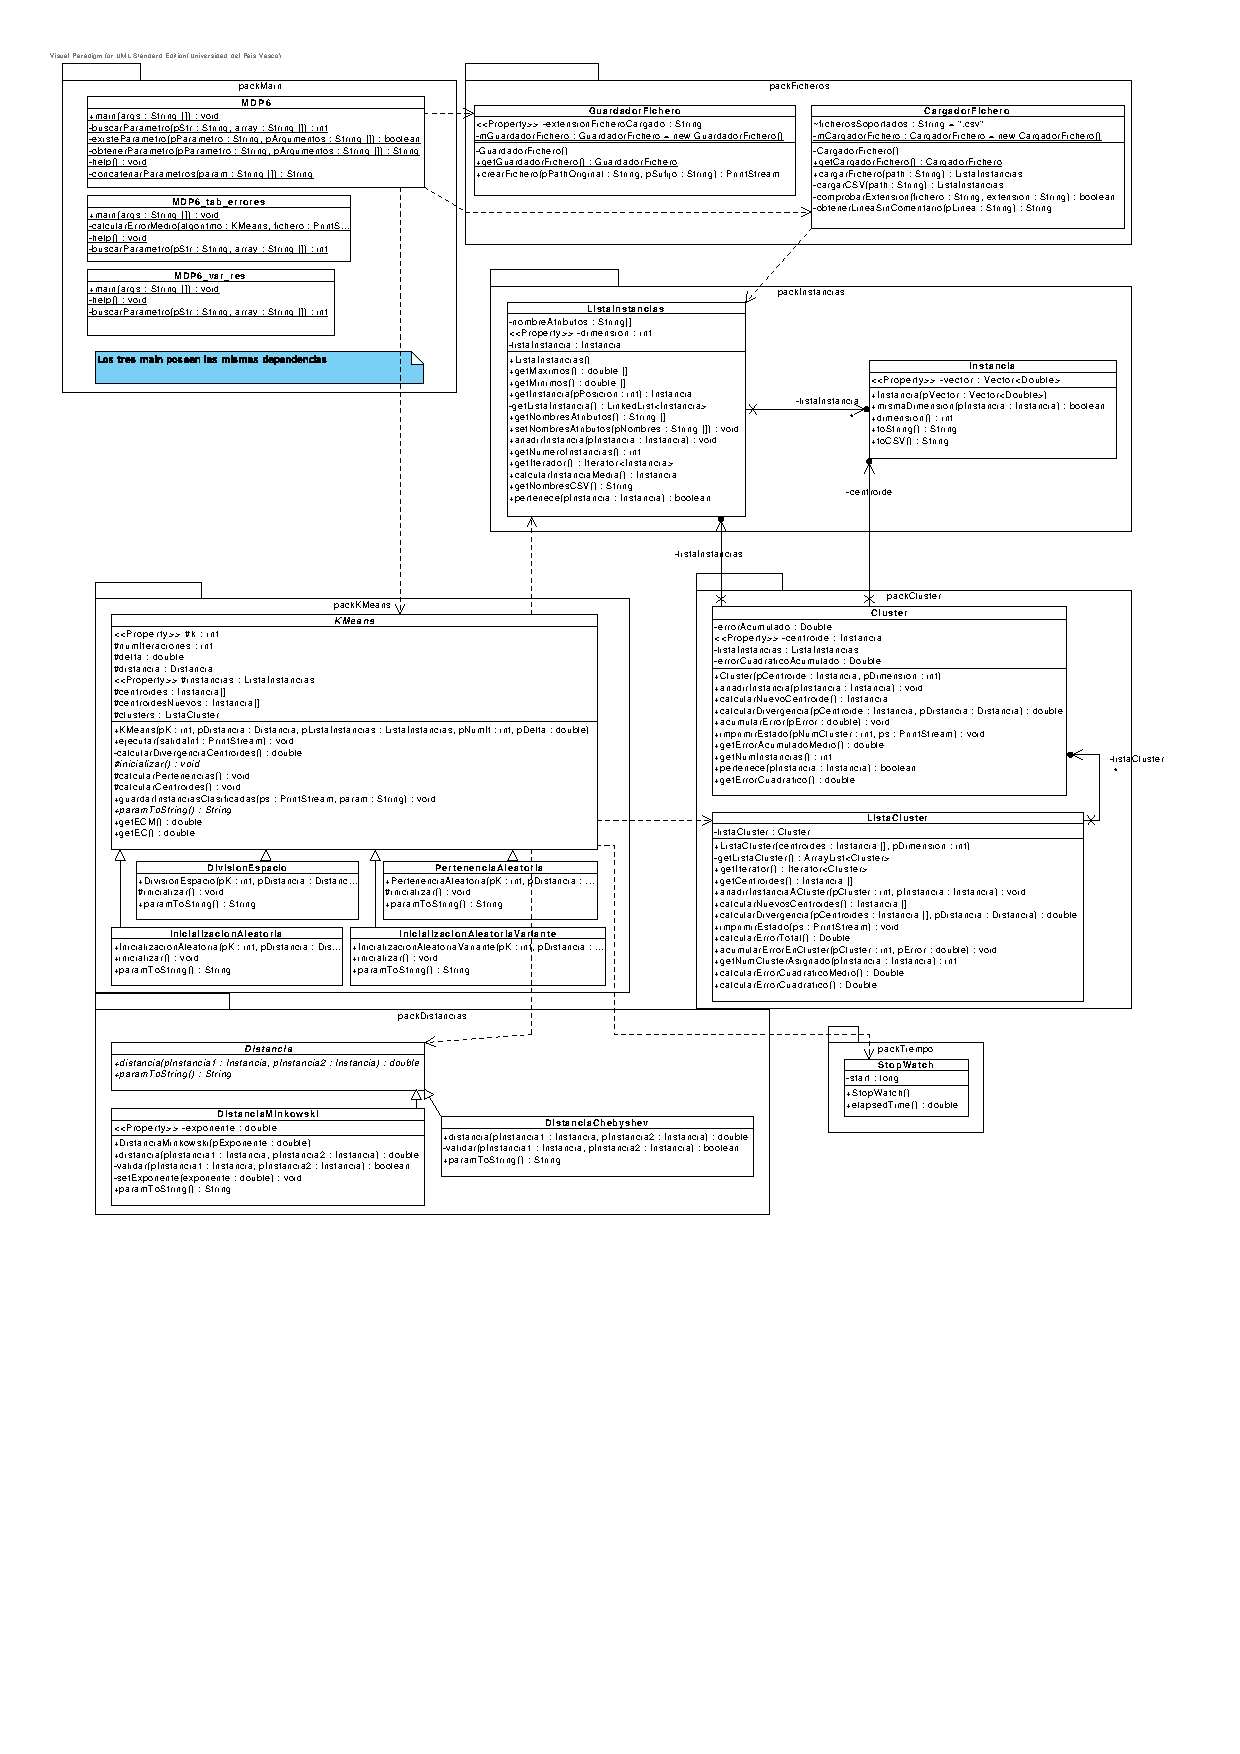
\includegraphics[width=1.1\textwidth, clip=true,trim=1cm 8cm 1.2cm 1cm]{./Figuras/clases.pdf}
	\caption{Diagrama de clases y paquetes}
	\label{fig:clases}
\end{figure}

\chapter{Resultados experimentales}

	\section{Banco de pruebas para la validación de software y resultados}
	
	Para la validación de nuestro software, MDP6, utilizaremos el software Weka usado en la asignatura. Ambos softwares, el propio y Weka, difieren en capacidad y soporte de funciones. Para la realización de pruebas, describimos las capacidades de cada uno de ellos:
	
	
	\begin{center}
		\textbf{MDP6}
	\end{center}
	
	\begin{itemize}
		\item	\textbf{Inicializaciones}. Disponemos de 4 tipos de inicializaciones diferentes:
			\begin{itemize}
			\item	\textbf{Inicialización aleatoria}. Elige al azar k instancias del conjunto de datos para actuar de centroides.
			\item	\textbf{Inicialización por petenencia aleatoria}. Por cada instancia, la incluye al azar en uno de los k clusters. Posteriormente se calculan los centroides.
			\item	\textbf{Inicialización por generación aleatoria de centroides}. Se recogen los rangos en que varían los atributos de todas las instancias. Posteriormente se crean k centroides con valores al azar incluidos en los diferentes intervalos identificados.
			\item	\textbf{Inicialización por división de espacio}. Se divide el espacio muestral de acuerdo al número de clusters a crear y se identifican los centroides.
			\end{itemize}
			
		\item	\textbf{Distancias}. Se han implementado dos tipos de métricas capaces de trabajar con el algoritmo
			\begin{itemize}
			\item	\textbf{Distancia Minkowski}. Implementada para cualquier valor del parámetro \textit{m} (siempre que sea un real positivo mayor o igual de 1).
			\item	\textbf{Distancia Chebyshev}.
			\end{itemize}
			
		\item	\textbf{Criterio de parada}. Se ofrece la posibilidad de establecer un límite de iteraciones para la ejecución del algoritmo o bien el uso de un valor a satisfacer para la divergencia entre conjuntos de centroides de dos iteraciones diferentes. También se pueden combinar ambos valores de forma que el primero en satisfacerse determine el fin del algoritmo.
		
		\item	\textbf{Tipos de atributos}. Únicamente se permiten valores numéricos y conocidos para los atributos de las instancias. Todo fichero que vaya a ser cargado debe satisfacer esta condición. No se ofrece funcionalidad como la normalización de atributos.
		
		\item	\textbf{Medidas de calidad}. Como medida del error tras el proceso de clustering se ofrece tanto el \textbf{Error Cuadrático} como el \textbf{Error Cuadrático Medio}.
		
		\item	\textbf{Clasificación de instancias}. Se puede generar un archivo conteniendo las instancias cargadas (en el mismo orden al de entrada) en formato CSV. En este fichero de salida, a cada instancia se le ha añadido un atributo que indica el cluster al que finalmente fue asociada tras la ejecución del algoritmo.
		
		\item	\textbf{Repetición de pruebas}. Como se explicará posteriormente, las pruebas realizadas con tipos de inicializaciones que utilicen generación de valores aleatorios no pueden ser repetidas ya que los valores variarán en cada ejecución.
	\end{itemize}
	
	\begin{center}
		\textbf{Weka}
	\end{center}
	
	\begin{itemize}
		\item	\textbf{Inicializaciones}. No ofrece más que un tipo de inicialización.
		
		\item	\textbf{Distancias}. Las distancias disponibles para el algoritmo son Minkowski 1 y Minkowski 2 (Euclídea y Manhattan respectivamente). Además, cada una de estas dos distancias permite normalizarlas.
		
		\item	\textbf{Criterio de parada}. Permite establecer el número máximo de iteraciones que realizará el algoritmo.
		\item	\textbf{Tipos de atributos}. Soporta nominales, numéricos, binarios, unarios, con valores desconocidos o nominales vacíos.
		\item	\textbf{Medidas de calidad}. En el caso de la distancia \textbf{Euclídea}, se ofrece el \textbf{Error Cuadrático} como medida de error. En el caso de la distancia \textbf{Manhathan}, la medida ofrecida es la \textbf{suma de las distancias dentro del cluster}.
		\item	\textbf{Clasificación de instancias}. Tras ejecutar el algoritmo, se puede visualizar el resultado de la agrupación de las instancias y guardarlas en formato \textbf{ARFF} con un atributo más correspondiente al cluster con que la instancia ha sido asociada.
		
		\item	\textbf{Repetición de pruebas}. Weka permite que para una misma semilla (parámetro configurable) los valores generados carezcan de variación, de forma que se puede repetir el mismo experimento una y otra vez para una misma semilla.
	\end{itemize}
	
	Los ficheros utilizados como fuente de instancias han sido \textbf{previamente procesados} con \textit{Weka} para adaptarlos a nuestro software. Se ha procedido a \textbf{eliminar el atributo clase} en aquellos ficheros que la tuvieran y se han guardado las instancias en \textbf{formato CVS}.
	
	Así mismo, en algunos casos ha sido necesario utilizar además un \textbf{procesador de texto} para poder obtener los resultados deseados. También se ha usado el software \textbf{R} para obtener ciertos resultados estadísticos y realizar comparaciones de valores. Para automatizar el proceso de obtención de datos, se han desarrollado programas \textbf{JAVA} extra y se ha utilizado un script del interprete \textbf{BASH}.
	
	Para la representación de resultados se ha utilizado el software \textbf{LibreOffice Calc} y la extensión \textbf{calc2latex} para generar el código Latex de las tablas presentes en este informe.
	
	\subsection{Pruebas realizadas}
	
	Se han realizado tres tipos diferentes de pruebas para comprobar la validez y rendimiento del software desarrollado. En cada una de estas pruebas los indicadores de referencia utilizados han sido:
	
		\begin{itemize}
			\item	\textbf{Medidas de error}. Comparación directa del error generado en el proceso de clustering. Prueba desarrollada en el apartado \ref{rescomparativos}, se utiliza el \textbf{Error Cuadrático} para realizar comparar directamente el software con Weka.
			
			\item	\textbf{Medidas de precisión}. Comparación de la \textbf{precisión} capaz de alcanzar nuestro software con la que Weka es capaz de alcanzar. El proceso se desarrolla y explica en el apartado \ref{resprecision}.
			
			\item	\textbf{Medidas estadísticas}. Uso de medidas como máximo, mínimo, media y varianza de un conjunto de datos para determinar la variabilidad de las repeticiones sucesivas de un determinado experimento con nuestro software. Proceso desarrollado en el apartado \ref{resestadisticos}.
		\end{itemize}
	
	\section{Resultados comparativos}
	\label{rescomparativos}
	En este apartado comparamos el software implementado con el algoritmo Kmeans de Weka por medio del error cuadrático. Este indicador de error solo se muestra en Weka al utilizar la distancia Euclídea, por lo tanto las comparaciones se limitan a este tipo de distancia. Además, nuestro software no es capaz de normalizar las instancias, así que desactivaremos esta opción al trabajar con Weka.
	
	En cuanto al resto de parámetros, para cada uno de los ficheros de pruebas se ha variado el parámetro \textbf{K} en el conjunto \{2,3,5,7,9\}. Por otro lado, el tipo de inicialización en Weka es único, pero con nuestro software hemos utilizado las 4 posibles.
	
	Otro dato a tener en cuenta es la gran dificultad de repetir un mismo resultado, para una misma configuración de parámetros, en nuestro software por el uso de aleatorios. Esto genera el problema de comparar el error variable de nuestro software con el de Weka.
	
	Para solucionarlo, hemos hecho 100 ejecuciones de cada combinación de parámetros posible y hemos utilizado la media de los diferentes errores obtenidos para conseguir un valor más estable del error cometido por nuestro software. El proceso con el ejecutable estándar desarrollado sería muy costoso, así que hemos desarrollado el programa \textit{MDP6\_tab\_errores.jar} para automatizar dicho proceso.
	
	Los ficheros correspondientes a este apartado están disponibles en la carpeta \textit{/resultados/resultados\_comparativos}. Se encuentran los ficheros originales, los ficheros operativos y los fichero resultado obtenidos. El resumen de los resultados se encuentra a continuación.
	
	
	\begin{figure}[htbp]
	\begin{center}
	\scalebox{0.8}{
	\begin{tabular}{|l|r|r|r|r|r|}
	\hline
	Error Cuadrático & Inic\_aleatoria & Pertenencia\_aleatoria & Cent\_aleatorios & División\_espacio & Weka \\ \hline
	K = 2 & 17.022.812.094,779 & 16.662.529.293,188 & 16.662.595.771,055 & 16.662.529.293,188 & 16.662.529.293,188 \\ \hline
	K = 3 & 15.367.892.995,782 & 15.308.965.075,088 & 15.276.313.379,049 & 15.068.933.772,772 & 15.347.180.933,720 \\ \hline
	K = 5 & 13.194.207.465,418 & 13.100.202.144,746 & 13.055.014.852,916 & 14.786.712.947,628 & 13.128.804.126,107 \\ \hline
	K = 7 & 11.748.015.592,402 & 11.590.997.272,742 & 11.685.296.452,310 & 13.886.614.328,470 & 12.208.057.266,416 \\ \hline
	K = 9 & 10.626.841.728,292 & 10.711.671.635,239 & 10.678.692.422,634 & 13.537.274.017,576 & 11.151.380.874,620 \\ \hline
	\end{tabular}
	}
	\end{center}
	\caption{Error cuadrático para el fichero colon.arff. Distancia Euclídea}
	\label{rescompcolon}
	\end{figure}
	
	
	\begin{figure}[htbp]
	\begin{center}
	\scalebox{0.9}{
	\begin{tabular}{|l|r|r|r|r|r|}
	\hline
	Error Cuadrático & Inic\_aleatoria & Pertenencia\_aleatoria & Cent\_aleatorios & División\_espacio & Weka \\ \hline
	K = 2 & 218.924,945 & 209.417,829 & 210.407,601 & 202.489,423 & 202.489,423 \\ \hline
	K = 3 & 119.441,033 & 108.167,063 & 107.651,418 & 110.504,153 & 110.504,153 \\ \hline
	K = 5 & 55.416,837 & 52.625,441 & 52.134,900 & 36.139,549 & 35.296,151 \\ \hline
	K = 7 & 36.428,538 & 39.363,275 & 40.904,587 & 35.296,151 & 15.905,814 \\ \hline
	K = 9 & 23.140,147 & 29.075,157 & 31.384,815 & 24.104,840 & 10.600,845 \\ \hline
	\end{tabular}
	}
	\end{center}
	\caption{Error cuadrático para el fichero food.arff. Distancia Euclídea}
	\label{rescompfood}
	\end{figure}
	
	
	\begin{figure}[htbp]
	\begin{center}
	\scalebox{0.92}{
	\begin{tabular}{|l|r|r|r|r|r|}
	\hline
	Error Cuadrático & Inic\_aleatoria & Pertenencia\_aleatoria & Cent\_aleatorios & División\_espacio & Weka \\ \hline
	K = 2 & 152,369 & 152,369 & 152,369 & 152,369 & 152,369 \\ \hline
	K = 3 & 92,647 & 96,026 & 91,888 & 145,279 & 78,941 \\ \hline
	K = 5 & 52,882 & 58,886 & 60,564 & 680,824 & 53,007 \\ \hline
	K = 7 & 41,422 & 51,064 & 51,155 & 680,824 & 38,926 \\ \hline
	K = 9 & 33,432 & 46,544 & 45,872 & 680,824 & 28,474 \\ \hline
	\end{tabular}
	}
	\end{center}
	\caption{Error cuadrático para el fichero iris.arff. Distancia Euclídea}
	\label{rescompiris}
	\end{figure}
	

	
	
	\FloatBarrier
	\section{Clasificación supervisada respecto de otro software de referencia}
	\label{resprecision}
	En este apartado observamos el cluster asignado a cada instancia de un fichero por ambos softwares comparándolo con la clase que la instancia tenía en el fichero original. El objetivo es obtener la tasa de aciertos que los diferentes softwares son capaces de alcanzar.
	
	En este caso no se han tenido en cuenta la variabilidad de los resultados de nuestro software y se ha comparado el de una sola ejecución.
	
	En cuanto a parámetros, se han tenido en cuanta las diferentes inicializaciones de nuestro software y varias distancias de las soportadas. En Weka se han utilizado las dos distancias soportadas (Manhattan y Euclídea) y por cada una se ha probado con y sin normalización.En cuanto al parámetro K, se establece igual al número de clases diferentes del fichero original. Estas pruebas se han basado en el fichero \textit{iris.arff}, por lo que el valor de K usado ha sido \textbf{3}.
	
	Para obtener las instancias etiquetadas en nuestro software se ha utilizado el ejecutable \textit{MDP6.jar} que automáticamente genera un fichero conteniendo las diferentes instancias y su cluster correspondiente. La variación de parámetro se ha llevado a cabo mediante un script BASH, \textit{MDP6\_param\_variator.sh},  con el que hemos obtenido los diferentes ficheros resultados.
	
	En el caso de Weka, el proceso se ha realizado de forma manual mediante su interfaz, ya que eran solo 4 las diferentes combinaciones de parámetros a probar.
	
	Para realizar la comparación con el fichero original de instancias ha sido preciso reetiquetar los valores de la clase estimados de forma que las clases se correspondieran en la mejor medida posible al fichero original. El fichero original también ha sido procesado para la comparación, variando el formato a CSV y cambiando el valor nominal de las clases por un valor numérico.
	
	Los ficheros resultado de este experimento se encuentran en \textit{/resultados/clasificación\_supervisada}, siguiendo la misma estructuración que los del apartado anterior.
	
	\begin{figure}[htbp]
		\begin{center}
			\begin{tabular}{|l|l|l|l|r|r|r|}
				\hline
				\textbf{Software} & \textbf{Inicialización} & \textbf{Distancia} & \textbf{Norm} & \multicolumn{1}{l|}{\textbf{\% aciertos}} & \multicolumn{1}{l|}{\textbf{\% errores}} & \multicolumn{1}{l|}{\textbf{E cuad}} \\ \hline
				Weka & Aleatoria & Minkowski 1 & False & 88,67 & 11,33 & 159,3 * \\ \hline
				Weka & Aleatoria & Minkowski 1 & True & 89,33 & 10,67 & 47,779 * \\ \hline
				Weka & Aleatoria & Minkowski 2 & False & 88,67 & 11,33 & 78,94 \\ \hline
				Weka & Aleatoria & Minkowski 2 & True & 89,33 & 10,67 & 7 \\ \hline
				MDP6 & Aleatoria & Minkowski 1 & False & 88,67 & 11,33 & 223,21 \\ \hline
				MDP6 & Aleatoria & Minkowski 2 & False & 88,67 & 11,33 & 78,95 \\ \hline
				MDP6 & Aleatoria & Minkowski 7'5 & False & 88,67 & 11,33 & 50,06 \\ \hline
				MDP6 & Aleatoria & Chebyshev & False & 88,67 & 11,33 & 82,2 \\ \hline
				MDP6 & Pert\_aleatoria & Minkowski 1 & False & 88,67 & 11,33 & 223,21 \\ \hline
				MDP6 & Pert\_aleatoria & Minkowski 2 & False & 89,33 & 10,67 & 78,95 \\ \hline
				MDP6 & Pert\_aleatoria & Minkowski 7'5 & False & 88,67 & 11,33 & 50,06 \\ \hline
				MDP6 & Pert\_aleatoria & Chebyshev & False & 66,67 & 33,33 & 48,36 \\ \hline
				MDP6 & Cent\_aleatorios & Minkowski 1 & False & 88,67 & 11,33 & 223,21 \\ \hline
				MDP6 & Cent\_aleatorios & Minkowski 2 & False & 66,67 & 33,33 & 78,94 \\ \hline
				MDP6 & Cent\_aleatorios & Minkowski 7'5 & False & 88,67 & 11,33 & 50,08 \\ \hline
				MDP6 & Cent\_aleatorios & Chebyshev & False & 51,33 & 48,67 & 87,51 \\ \hline
				MDP6 & Div\_espacio & Minkowski 1 & False & 88,67 & 11,33 & 223,21 \\ \hline
				MDP6 & Div\_espacio & Minkowski 2 & False & 66,67 & 33,33 & 145,28 \\ \hline
				MDP6 & Div\_espacio & Minkowski 7'5 & False & 66,67 & 33,33 & 91,2 \\ \hline
				MDP6 & Div\_espacio & Chebyshev & False & 66,67 & 33,33 & 87,51 \\ \hline
			\end{tabular}
			
		\end{center}
		*Sum of within clusters distances.
		\caption{Resultados de clasificación para el fichero iris.arff}
		\label{resiris_clasificacion}
	\end{figure}
	
	
	En este caso los resultados son bastante similares los unos a otros, la mayoría de casos fallan 17 instancias de clasificación, un 8.6\%. La única ejecución que obtiene una mayor tasa de aciertos es la realizada mediante centroides aleatorios para tres clusteres y sobre distancia euclídea que resulta en solo 16 fallos. Por lo demás, existe también un gran grupo de resultados que aciertan 100 instancias nada más, cuestión que puede deberse a la limitación de iteraciones o a un mal resultado en la selección aleatoria de centroides iniciales que resultan en una convergencia no deseable.
	
	
	\FloatBarrier
		
	\section{Variabilidad de los resultados}
	\label{resestadisticos}
	Este apartado se dedica única y exclusivamente a la observación de la variabilidad de los resultados de una ejecución a otra, con los mismos parámetros, de nuestro software.
	
	Las pruebas se han realizado con el uso de la distancia Euclídea, variando el parámetro K en el conjunto \{3, 5, 8\} y la inicialización entre las 4 posibilidades disponibles.
	
	Para cada una de las combinaciones de parámetros tratadas,  se ha ejecutado 10000 veces, obteniéndose en cada una el valor del error cuadrático medio.
	
	El proceso se ha automatizado y ejecutado mediante el ejecutable \textit{MDP6\_var\_res.jar}, desarrollado especialmente para la tarea.
	
	Posteriormente, los 10000 valores de cada ejecución se han tratado con el software R para obtener  las medidas estadísticas deseadas.
	
	Los ficheros resultado de este experimento se encuentran en \textit{/resultados/variabilidad\_resultados}, siguiendo la misma estructuración que los del apartado \ref{rescomparativos}. A continuación se muestran los resultados obtenidos.
	
	
	\begin{figure}[htbp]
	\begin{center}
	\begin{tabular}{|c|l|r|r|r|}
	\hline
	\multicolumn{1}{|l|}{\textbf{\textit{}}} & \multicolumn{1}{c|}{\textbf{\textit{K=}}} & \multicolumn{1}{c|}{\textbf{\textit{3}}} & \multicolumn{1}{c|}{\textbf{\textit{5}}} & \multicolumn{1}{c|}{\textbf{\textit{8}}} \\ \hline
	\multicolumn{ 1}{|c|}{\textbf{\textit{Inicialización aleatoria}}} & Mínimo & 3794 & 1274 & 362,8 \\ \cline{ 2- 5}
	\multicolumn{ 1}{|c|}{} & 1er Cuadrante & 3815 & 1902 & 539,8 \\ \cline{ 2- 5}
	\multicolumn{ 1}{|c|}{} & Mediana & 4093 & 2019 & 1452,2 \\ \cline{ 2- 5}
	\multicolumn{ 1}{|c|}{} & Media & 4349 & 2123 & 1112,8 \\ \cline{ 2- 5}
	\multicolumn{ 1}{|c|}{} & 3er Cuadrante & 4093 & 2154 & 1504 \\ \cline{ 2- 5}
	\multicolumn{ 1}{|c|}{} & Máximo & 7039 & 5775 & 5678,4 \\ \cline{ 2- 5}
	\multicolumn{ 1}{|c|}{} & Varianza & 925665,7 & 478596,4 & 250481,7 \\ \hline
	\multicolumn{ 1}{|c|}{\textbf{\textit{Pertenencia aleatoria}}} & Mínimo & 7039 & 1274 & 378,4 \\ \cline{ 2- 5}
	\multicolumn{ 1}{|c|}{} & 1er Cuadrante & 3794 & 1827 & 876,5 \\ \cline{ 2- 5}
	\multicolumn{ 1}{|c|}{} & Mediana & 3815 & 1964 & 1519,1 \\ \cline{ 2- 5}
	\multicolumn{ 1}{|c|}{} & Media & 4093 & 1908 & 1292,3 \\ \cline{ 2- 5}
	\multicolumn{ 1}{|c|}{} & 3er Cuadrante & 3997 & 2024 & 1658,4 \\ \cline{ 2- 5}
	\multicolumn{ 1}{|c|}{} & Máximo & 4093 & 3395 & 2441,9 \\ \cline{ 2- 5}
	\multicolumn{ 1}{|c|}{} & Varianza & 57161,97 & 1274 & 235878,9 \\ \hline
	\multicolumn{ 1}{|c|}{\textbf{\textit{Centroides aleatorios}}} & Mínimo & 3794 & 115044,2 & 378,4 \\ \cline{ 2- 5}
	\multicolumn{ 1}{|c|}{} & 1er Cuadrante & 3815 & 1827 & 876,5 \\ \cline{ 2- 5}
	\multicolumn{ 1}{|c|}{} & Mediana & 4093 & 1964 & 1513,4 \\ \cline{ 2- 5}
	\multicolumn{ 1}{|c|}{} & Media & 3992 & 1914 & 1277,4 \\ \cline{ 2- 5}
	\multicolumn{ 1}{|c|}{} & 3er Cuadrante & 4093 & 2024 & 1653,7 \\ \cline{ 2- 5}
	\multicolumn{ 1}{|c|}{} & Máximo & 6655 & 3483 & 2441,9 \\ \cline{ 2- 5}
	\multicolumn{ 1}{|c|}{} & Varianza & 50895,6 & 1339 & 236035,2 \\ \hline
	\multicolumn{ 1}{|c|}{\textbf{\textit{División espacial}}} & Mínimo & 4093 & 118689,5 & 1129 \\ \cline{ 2- 5}
	\multicolumn{ 1}{|c|}{} & 1er Cuadrante & 4093 & 1339 & 1129 \\ \cline{ 2- 5}
	\multicolumn{ 1}{|c|}{} & Mediana & 4093 & 1339 & 1129 \\ \cline{ 2- 5}
	\multicolumn{ 1}{|c|}{} & Media & 4093 & 1339 & 1129 \\ \cline{ 2- 5}
	\multicolumn{ 1}{|c|}{} & 3er Cuadrante & 4093 & 1339 & 1129 \\ \cline{ 2- 5}
	\multicolumn{ 1}{|c|}{} & Máximo & 4093 & 1339 & 1129 \\ \cline{ 2- 5}
	\multicolumn{ 1}{|c|}{} & Varianza & 0 & 0 & 0 \\ \hline
	\end{tabular}
	\end{center}
	\caption{Medidas estadísticas para las diferentes pruebas}
	\label{tablavar}
	\end{figure}
	
	
	
	Los resultados obtenidos por los algoritmos en los que intervienen variables de carácter aleatorio arrojan resultados distintos en cada repetición mientras que el algoritmo de inicialización por división del espacio resulta siempre en un resultado idéntico siempre que tratemos con el mismo fichero de datos.
	
	La distribución de los resultados se muestra gráficamente mediante franjas en los valores en los que tienen tendencia a converger los resultados de la aplicación de los algoritmos. Estas franjas son similares entre el algoritmo de pertenencia aleatoria y el de centroides aleatorios.
	
	\begin{figure}
		\centering
		\includegraphics[width=0.7\linewidth]{Figuras/Franjas}
		\caption{Franjas de convergencia}
		\label{fig:Franjas}
	\end{figure}

	
	Si comparamos los índices estadísticos, observamos que los algoritmos que mejor puntúan en base a su media son los de pertenencia y centroides aleatorios para aquellas pruebas realizadas sobre 3 y 5 clusters, sin embargo, la puntuación de la inicialización aleatoria es mejor para 8 clusters.
	
	La división del espacio otorga siempre el mismo resultado teniendo por tanto varianza cero. Este algoritmo no ha puntuado como último en ninguna de las pruebas por lo que podría ser un candidato a cota realista del desempeño posible. Por otra parte, en el caso de k=3 encontramos curioso el hecho de que todas las medianas sean iguales y coincida exactamente con el resultado arrojado por la división del espacio. Esto se puede deber a que el algoritmo converja en un valor de 4093 para una gran cantidad de condiciones iniciales distintas siendo esta cifra ,por tanto , un atractor clásico.

	El algoritmo que mayor varianza arroja en todos los experimentos ha sido el de inicalización aleatoria siendo la varianza de los otros dos algoritmos evaluables en función de este parámetro similar entre si. Pese a tener la tendencia a arrojar un mejor resultado con un número grande de clusters hay que tener en cuenta esta gran variabilidad de resultados para el algoritmo de inicialización aleatoria.
	
	También parece claro que un mayor número de clusters favorece una disminución de la varianza para el algoritmo de inicialización aleatoria. Esto tiene sentido si entendemos que a mayor número de clusters la distancia de las distintas instancias al centroide del cluster es menor en comparativa y dado que seleccionamos una instancia como centroide, es más probable que exista una convergencia rápida.
	
	Sin embargo, para los algoritmos de pertenencia aleatoria y centroides aleatorios parece que sucede al contrario esto puede deberse al hecho de que las pruebas se han realizado sobre un número limitado de iteraciones siendo estos dos algoritmos de convergencia más lenta.
	\section{Análisis crítico y discusión de resultados}
	Los resultados de la aplicación de este programa sobre los datos de prueba han sido variados y complejos en muchos casos. La gran variedad de parámetros de entrada establece una gran forma de realizar múltiples pruebas de precisión consiguiendo en muchos casos unos resultados que resultan óptimos siempre y cuando seamos capaces de adaptar los parámetros del programa a las necesidades del conjunto de instancias estudiadas.
	
	Los diferentes algoritmos de inicialización ofrecen distintas características a tener en cuenta. Para algunos algoritmos encontramos que funcionan mejor comparativamente para aquellas situaciones en las que menos clusters haya, tal es así en el caso de los centroides aleatorios y la pertenencia aleatoria. 
	
	Sin embargo, se da la circunstancia de que para una mayor cantidad de clusters el algoritmo de inicialización que parece adaptarse mejor es el clásico de inicialización aleatoria.
	
	Este no es el único parámetro a tener en cuenta ya que también conviene estudiar la varianza de las distintas inicializaciones para considerar si lo que se busca es una solución precisa a la vez que estable. La cantidad de atributos influye también en la selección del método de inicialización ya que ciertos algoritmos tienen una mayor precisión comparativa cuando se aumenta el número de dimensiones\footnote{Hecho que aún no hemos estudiado en profundidad}.
	
	Por otro lado, el software desarrollado comparado con el programa \textbf{Weka}, con el que trabajamos en clase, arroja resultados similares, en ciertas ocasiones mejores y en otras peores debido sobre todo a que con la variedad de posibilidades que implementa nuestro software somos capaces de adaptarnos mejor a las situaciones que plantean los distintos espacios en estudio.
	
	Por último, cabe señalar la cantidad de resultados reseñables que hemos sido capaces de alcanzar gracias al estudio en masa de los resultados proporcionados, estos resultados no siempre están reflejados en la práctica por ser resultados parciales e intermedios.
	\section{Rendimiento del software}
	El software desarrollado posee una complejidad computacional que difiere en función del algoritmo de inicialización. El algoritmo de clustering que usamos, por si mismo, posee un orden computacional $kn$ siendo k el número de iteraciones que realiza el software y n el número de instancias en evaluación.
	
	Para las inicializaciones de centroide aleatorio, división del espacio e inicialización aleatoria, el software no necesita recorrer las instancias que se encuentran en evaluación, sin embargo, para el de pertenencia aleatoria es necesario acceder a todas estas instancias.
	
	Esta necesidad de acceso no varía el orden de magnitud aunque aplicado al algoritmo tenemos que el orden resultante es de $k(1+n)$ interpretando las variables de la misma forma que el enunciado anterior.
	
	Dicho esto, el algoritmo en cualquiera de sus vertientes y sobre los archivos de prueba que hemos usado, aún en el caso de realización sistemática de experimentos, no ha presentado ningún inconveniente temporal. Este rendimiento podría ser evaluado de nuevo sobre archivos con una mayor cantidad de información para conocer realmente en qué cotas es inviable su aplicación y debería ser reestructurado siguiendo criterios de rendimiento.

\chapter{Conclusiones}

\section{Motivación para la realización de \textit{Clustering}}

Explorar un conjunto de instancias con el objetivo de crear agrupaciones (clusters) donde todas tienen algo en común, alguna característica similar.

Hay diferentes estrategias a considerar. Si, por ejemplo, queremos clasificar datos, digamos 1000 instancias, en tres clases diferentes sin tener que examinarlas una por una, podemos hacer clustering k-medias con k = 3, y obtendríamos directamente los tres grupos. Como contrapartida, puede que muchas instancias hayan quedado mal clasificadas en la clase que no le corresponde. Este es el enfoque que hemos llevado en el desarrollo de nuestro software.

En este mismo ejemplo, otra opción es crear más clusters, digamos 10. Posteriormente, podríamos examinar una instancia de cada cluster (o dos o tres para tener más certeza) de forma  que a todas las instancias de ese cluster les asignamos la clase resultante de esa instancia. De esta forma se reducen los errores al etiquetar las 1000 instancias, pero en vez de examinarlas todas, únicamente se deben examinar 10, 20 o 30 de las 1000 instancias originales.

\section{Conclusiones de los resultados}

El software desarrollado es \textbf{válido}, cuanto menos, realiza el mismo trabajo que Weka, \textbf{mejorándolo} en algunos casos, si bien las instancias de trabajo están \textbf{limitadas} a aquellas definidas por atributos \textbf{numéricos}.

A destacar el hecho de que, en el experimento de clasificación supervisada, las diferentes combinaciones de parámetros obtengan la misma tasa de aciertos. Si bien es un hecho que no sabemos explicar muy bien, también es cierto que en la prueba nos hemos limitado al fichero \textit{iris} sin probar otras opciones.

\section{Conclusiones generales}

El tiempo invertido en el proyecto ha sido mucho mayor conforme se acercaba la fecha de entrega original. Debemos mejorar en organización, especialmente al principio de la práctica, donde un diseño poco especificado con ciertas cosas \textit{"en el aire"} nos llevaron a diseñar al implementar.

También el hecho de probar y perfeccionar el funcionamiento de \textbf{todo} el código antes de comenzar con la extracción de resultados experimentales nos limitó en el análisis de los mismos y en la retroalimentación del algoritmo implementado.

Resumiendo, hay que mejorar la planificación, dividir el proyecto en partes para poder mejorarlo incrementalmente.

Pese a los problemas, la solución implementada ofrece una variedad bastante amplia de parámetros posibles a utilizar, teniendo 4 tipos de inicialización, dos métricas diferentes - en el caso de la métrica Minkowski ofrece otro parámetro más que variar- y la posibilidad de controlar el número de iteraciones tanto por la especificación de un máximo de vueltas, como por la especificación del margen de variación que se debe alcanzar hasta dar por válidos los centroides identificados.

La semana extra de trabajo nos ha servido para exponer resultados útiles que ayuden a determinar la calidad de nuestro software, resultados para los cuales se ha observado la gran utilidad que tiene la automatización de la obtención de las mismas para ser capaces de procesar un gran volumen de datos obteniendo los resumen concluyentes.

\section{Propuestas de mejora}

La entrada a nuestro programa es un factor un tanto restrictivo en el sentido de que el único tipo de fichero soportado es el \textbf{CSV}. Inicialmente, la intención era implementar también la carga de ficheros \textbf{ARFF}, que no ha sido posible hacerla por falta de planificación principalmente.

En cuanto a inicializaciones, hemos implementado 4 tipos diferentes. De los tres, el correspondiente a la división de espacio es el que más puede mejorar, ya que para su implementación no hemos llegado a consultar bibliografía extra. El mapeo de aleatorios sería otra mejora que garantizaría estabilidad a tres de las inicializaciones.

Una restricción que podríamos eliminar está asociada al tipo de datos tratados, el algoritmo solo es capaz de lidiar con atributos de tipo numérico, siendo imposible realizar la carga de instancias que contengan valores no numéricos. De hecho, algunos de los ficheros han tenido que ser preprocesados para poder trabajar con ellos.

También teníamos un problema con la representación de los resutados, ya que los valores reales se presentaban con todos los decimales que tuvieran. Esto fue solucionado en la semana extra, haciendo que al imprimir los valores, se redondeasen previamente a 3 o 5 decimales.

Se podrían mejorar los programas auxiliares creados, de forma que permitan configurar más parámetros (las Ks a usar por ejemplo) y permitan experimentar a los usuarios de la aplicación.

Por último, cabe mejorar el apartado de resultados del algoritmo utilizando métodos concretos de la evaluación de clusters. Por ejemplo, la implementación del índice silueta, que sería un indicador mejor que el error cuadrático y nos permitiría saber directamente lo bien o mal que nuestro algoritmo realiza el clustering.



%Bibliografía

\newpage
\bibliographystyle{plain}

\bibliography{mdp6}

\newpage


\chapter{Valoración subjetiva}
	
	\section*{Alcance de objetivos}
	Los objetivos de le práctica tal y como están definidos en este documento han sido cumplidos, no solo hemos sido capaces de comprender el funcionamiento de este algoritmo sino que además hemos sido capáces de implementarlo en la práctica y de proponer variaciones frente a lo estudiado en clase.
	\section*{Utilidad de la tarea}
	Esta tarea ha servido para que nos demos cuenta de nuestra capacidad de adaptación de lo aprendido en clase a un problema concreto que se nos plantea. Además, el hecho de que lo que se pedía realmente no tuviera un carácter cerrado ha hecho que pudieramos desarrollar un poco más en profundidad aquellas áreas que más nos atraían dentro de los parámetros establecidos.
	
	Por otra parte, dada la necesidad de evaluar nuestro trabajo desde un punto de vista objetivo, hemos aprendido también la forma en la que debemos presentar los resultados de una práctica de forma que podamos sacarle un mayor \emph{jugo} a todas las posibilidades que ofrece aquellos elementos desarrollados durante esta práctica.
	\section*{Dificultad}
	Dado que este es un trabajo de mínimos, la dificultad no es fácilmente mesurable. Cumplir los objetivos mínimos no nos ha supuesto un mayor problema, sin embargo, la necesidad de improvisar sobre estos mínimos ha supuesto un reto en la forma de planificar las adiciones que creyeramos oportunas de forma que fueran viables en el tiempo disponible.
	
	Otra dificultad que hemos tenido ha sido el hecho de habernos visto con un gran volumen de datos a analizar y poco tiempo para hacerlo, en este sentido nos deja mal sabor de boca el no haber acabado antes la implementación para poder analizar más a fondo los resultados obtenidos.
	\section*{Tiempo de trabajo}
	
	\begin{figure}[htbp]
	
		\begin{center}
			\begin{tabular}{|r|r|}
				\hline
				\textbf{Plazo inicial} & \multicolumn{1}{l|}{\textbf{Horas}} \\ \hline
				Diseño & 02:00:00 \\ \hline
				Implementación & 00:30:00 \\ \hline
				Trabajo con Weka & 02:30:00 \\ \hline
				Búsqueda bibliográfica y preparación & \multicolumn{1}{l|}{} \\ \hline
				Redacción de informe y generación de documentación & 07:00:00 \\ \hline
				Preparación del entorno de trabajo & 01:00:00 \\
				(repositorio GIT, estructuración de contenido) & \multicolumn{1}{l|}{} \\ \hline
				\textbf{Semana extra} & \multicolumn{1}{l|}{} \\ \hline
				Replanteamiento del plan de trabajo & 02:00:00 \\ \hline
				Implentación & 02:30:00 \\ \hline
				Obtención de resultados & 05:00:00 \\ \hline
				Redacción & 07:00:00 \\ \hline
			\end{tabular}
		\end{center}
			\caption{Horas invertidas en el proyecto}
		\label{horas}
	\end{figure}
	
	
	\section*{Sugerencias de mejora}
	
	\section*{Críticas}

\end{document}
